\documentclass[preprint,12pt,authoryear]{elsarticle}
\journal{Journal of Systems and Software}
\biboptions{authoryear,round}
\usepackage[T1]{fontenc}
\usepackage[utf8]{inputenc}
\usepackage{lmodern}
\usepackage{amsmath,amssymb,amsthm}
\usepackage{booktabs,longtable,array,tabularx}
\usepackage{graphicx}
\usepackage{float}
\usepackage{url}
\usepackage{xurl}
\usepackage{hyperref}
\usepackage{microtype}
\usepackage{enumitem}
\providecommand{\tightlist}{\setlength{\itemsep}{0pt}\setlength{\parskip}{0pt}}
\usepackage{siunitx}
\graphicspath{{./}}
\hypersetup{colorlinks=true,urlcolor=blue,citecolor=black,linkcolor=black}
\emergencystretch=3em

\begin{document}
\begin{frontmatter}
\title{When Can a Blockchain Monitor Make a Decision? Source-Audited Feature Readiness, Historical State, and Exact-Execution Evidence}
\author[aff1,aff2]{Oleksandr Kuznetsov\corref{cor1}}
\cortext[cor1]{Corresponding author. ORCID: 0000-0003-2331-6326.}
\ead{oleksandr.kuznetsov@uniecampus.it}
\address[aff1]{Department of Theoretical and Applied Sciences, eCampus University, Italy}
\address[aff2]{Department of Intelligent Software Systems and Technologies, School of Computer Science and Artificial Intelligence, V.~N. Karazin Kharkiv National University, Ukraine}
\begin{abstract}
A history-dependent blockchain monitor may fail because its feature is undefined, its observation boundary misses a relevant transfer, its score is not extreme, or its candidate is suppressed. We distinguish these states in a source-audited evaluation of Ethereum runtime monitoring. Four earlier incident families (Li.Fi, Revest, Bacon and Rari Fuse) provide five documented successful executions: a daily-reset token-outflow rank notifies none, while longer causal history yields exact known-execution notifications for Bacon and one Rari transaction. In a separate incident-derived frame, sixteen fixed component nominations were audited across 480 Ethereum emitter-days and 44,780 selected transactions; 410 days had fewer than twenty selected transactions, an upper-bound failure of the nineteen-prior-observation requirement. For twelve additional comparison contracts (714,951 observations), daily-reset z-score, positive-MAD and EWMA event-count features were defined for 38.50\%, 1.93\% and 99.52\%, respectively. Seven of the sixteen incident-derived nominees then underwent a complete source-linked transaction reconstruction: 525 selected transactions and 441 rank/count/grouping/budget configurations were independently reproduced. A count rule matched one documented Schnoodle exploit transaction in a 27-notification stream, whereas the historical rank remained ineligible; the other streams exhibited distinct boundary, warm-up and score constraints. This nonrandom, exploratory extension does not establish population recall or false-positive rates. The results motivate separate validation contracts for observation, causal feature computability, construct alignment, score extremeness and realized notification delivery.
\end{abstract}
\begin{keyword}
Blockchain monitoring \sep Runtime monitoring \sep Empirical software engineering \sep Feature readiness \sep Historical initialization \sep Reproducibility \sep Decentralized finance
\end{keyword}
\end{frontmatter}

\section{Introduction}\label{sec:intro}

An automated software monitor is meaningful only if the data required by its decision rule can be observed when the decision is due. This requirement precedes the numerical choice of score threshold and the allocation of notifications. In conventional runtime verification, monitoring semantics explicitly distinguish the trace that is available from a system property and from the monitor's answer \citep{Leucker2009RV,Bauer2011RV}. Streaming anomaly detectors similarly depend on warm-up rules and observational constraints \citep{Lavin2015NAB}. A detection-rate figure can conceal a monitor that was incapable of computing its intended feature on much of the evaluated workload.

This paper studies that failure mode in Ethereum decentralized finance (DeFi). A typical blockchain monitoring pipeline nominates observable smart-contract components, reads the events of transactions selected by those components, extracts features, updates state, evaluates an anomaly rule, groups related candidates and allocates a daily notification budget. A user-to-attacker transfer may bypass the selected component even if the attack transaction contains events emitted by that component. A monitor based on outflow from the selected contract is therefore neither equivalent to a transaction-wide exploit monitor nor a general-purpose security guarantee. The need to match security claims to threat mechanisms is emphasized in DeFi attack systematizations and transaction-level monitoring studies \citep{Zhou2023SoKDeFi,Wu2024DeFiRanger,Meng2026Houston}.

We first observed an adverse outcome for a fixed, history-dependent token-outflow rule in two externally acquired incidents: Li.Fi and Revest. Although every independently admitted execution was visible in the selected transaction observations, the rank rule generated no notification for these executions. A count-based rule produced one verified Li.Fi match. The immediate gating reason was insufficient positive same-token history under the declared daily state reset. This finding, by itself, is a diagnostic of a particular configuration rather than a new anomaly-detection method.

To assess whether the failure was confined to the originally examined transactions or was a property of the wider observation pipeline, we performed a label-free audit of all selected transactions and a full replay with alternate history retention. We then examined two additional, historically documented incident families, Bacon Protocol and Rari Fuse Pool~127, using source-bound transaction identities and separately indexed complete event bundles. Their observation boundaries were nominated before the new ranking outputs were generated but after the initial Li.Fi/Revest results were known. We disclose that exposure rather than describe the additional cases as a globally blind test.

Our principal question concerns \emph{software monitor validation}: at what stage does the monitor's input contract fail, and can the effects of a changed state-initialization policy be distinguished from the meaning of a security feature and from subsequent notification admission? We address three research questions:

\begin{description}
\item[RQ1 (feature readiness).] How frequently does the selected historical traffic supply enough strictly preceding same-token positive observations to compute a history-dependent rank? Does end-of-day traffic overstate readiness at the known execution time?
\item[RQ2 (initialization and dispatch).] Holding the observed transactions and decision rule fixed, how do three history-retention policies affect eligible scores, candidate notifications and exact matches to independently reviewed known executions? How does the count comparator behave on the same component view?
\item[RQ3 (construct validity).] Do gross token-outflow features on nominated core addresses correspond to the security-relevant mechanism of the documented exploit?
\end{description}

The work treats feature computability, attack-boundary alignment, and conditional rank extremeness as separate, testable preconditions for interpreting an automated monitor. A supplementary comparison-contract census evaluates the portability of event-count warm-up diagnostics, without treating the controls as labelled non-attacks. A separate source screen fixed sixteen incident-derived Ethereum emitter nominations from a version-pinned exploit catalogue before measuring their traffic. Seven nominated views subsequently underwent source-linked reconstruction and deterministic replay, while the remaining nine retain their original screening dispositions. The seven are not a random test set or seven newly admitted incident-wide detector-performance experiments. We provide a versioned, independently checked measurement procedure, contrasting historical-initialization outcomes, and a source-linked account of why event-count sufficiency and actual feature computability differ. The rank formula, minimum-history arithmetic and conventional budget policies are not claimed as novel. The reported numbers describe four incident families, five known successful executions across those families, and several overlapping Rari component views; they are not prevalence or generalizable detection-rate estimates. The protocol and independently verifiable artifacts establish what was measured and why the limitations matter for software-monitor validation \citep{Kitchenham2004Evidence,Wohlin2012Experimentation}.

\section{Related work and differentiation}\label{sec:related}

\paragraph{Runtime monitors and feature preconditions.} Runtime verification concerns the evaluation of properties over finite observations of an executing system \citep{Leucker2009RV,Bauer2011RV}. Our study does not verify a temporal-logic property or claim formal completeness. It measures a weaker, practical prerequisite: whether the data and pre-event state needed by a particular score exist at the time of the event. A missing feature is distinct from an observed low anomaly score. This distinction can be encoded as a monitor validation contract and verified without attack labels. Streaming evaluations such as NAB explicitly recognize the relevance of event time and detection windows \citep{Lavin2015NAB}; our unit of analysis is an exact blockchain transaction and a selected-core observation boundary.

\paragraph{DeFi exploit detection and semantics.} TXSPECTOR studies exploit patterns through transaction dependencies, EtherClue provides investigation-oriented indicators, and DeFiRanger models higher-level financial operations for price manipulation \citep{Zhang2020TxSpector,Aquilina2021EtherClue,Wu2024DeFiRanger}. HOUSTON evaluates richer protocol-level anomalies over a substantially larger collection of historical incidents \citep{Meng2026Houston}. These systems motivate why protocol semantics matter but cannot be compared numerically with our simple fixed-core rank and count rules: observation populations, labels and detection units differ. A method that observes ERC-20-shaped transfers at a nominated address need not model native ETH borrowing, user allowance abuse, or accounting invariants \citep{Vogelsteller2015ERC20,Revest2022Postmortem,Rari2022Postmortem}.

\paragraph{Event provenance and cross-chain monitoring.} XChainWatcher applies logic-driven event monitoring, whereas BridgeGuard studies detection of cross-chain attack transactions \citep{Augusto2025XChainWatcher,Wu2025BridgeGuard}. The Ethereum address-and-transaction observation model used here is narrower. The diamond proxy architecture relevant to Li.Fi also distinguishes an entrypoint's emitted logs from implementation facets and user token transfers \citep{Mudge2020ERC2535,BlockSec2022LiFi}. These considerations constrain any claim that a selected event trace represents all protocol activity.

\paragraph{Empirical security evaluation and artifacts.} Security-ML studies warn against unrealistic experimental populations, label assumptions and over-interpretation of numerical performance \citep{Sommer2010ClosedWorld,Arp2022Dons}. Empirical-software-engineering methodology recommends explicit experimental units and transparent inclusion rules \citep{Kitchenham2004Evidence,Wohlin2012Experimentation}. Hidden data dependencies and state configuration are also recognized as sources of operational technical debt \citep{Sculley2015Debt}. Our independent evidence records, exact hash bindings and source-tier distinctions aim to make such assumptions auditable. DeFiHackLabs supplies reproducible exploit \emph{candidate} code, not automatically complete inventories of all successful historical attacks \citep{DeFiHackLabs2026}. Forta documents practical monitoring interfaces but does not establish the performance of the particular rules tested here \citep{FortaDocs}.

The specific empirical observation is that numerical eligibility and actual notification coverage can respond differently to retaining historical state. The applicable outcome must be measured at the same transaction and component boundary; it does not follow from the elementary warm-up inequality alone. We distinguish the known-subset exact notifications from the far broader notion of incident-wide recall.

\section{Monitoring model and estimands}\label{sec:model}

\subsection{Observation boundary, chronology and input units}
For each incident family $c$, a predeclared component view $v$ specifies one or more Ethereum log-emitting addresses. A transaction is \emph{selected} when at least one successful observed log is emitted by a view address. The full log bundle of a selected transaction is used to derive token-flow features, including transfer events from other emitters; selection itself does not use an attack label, anomaly score or transfer amount. Selected transactions are ordered by block number and transaction index. The block timestamp is a logical historical event time, not an observed network delivery time.

A \emph{case family} is a documented exploit event, not a row in an experiment table. Its \emph{core view} is a monitored component, not a separate attack; the Rari fETH, fUSDC and Comptroller views belong to one family. A \emph{known execution} is a historically identified and separately reviewed transaction that executed the documented unauthorized behavior. The verified inventories used here are \texttt{KNOWN\_SUBSET\_ONLY}; neither the negative population nor all historical exploit transactions are completely adjudicated. Therefore an emitted alert on an unknown transaction is not a false positive and a reference denominator is not a full incident recall denominator.

The extracted ERC-20-shaped fields are gross integer quantities as represented in the event data; they do not independently establish token compliance or a native-asset state delta. For token $k$, $x_{i,k}>0$ denotes the gross external token outflow whose sender is in the nominated view and whose recipient is outside it, as defined by the frozen extractor. Inflows do not cancel outflows. Different tokens have independent histories and raw units cannot be added across tokens without an external unit conversion \citep{Vogelsteller2015ERC20}.

\subsection{Feature readiness and the rank rule}
Let $H_{i,k}^{(m)}$ be the up-to-128 most recent strictly preceding positive values for token $k$ available at selected transaction $i$ under history mode $m$. The reported rank is
\begin{equation}\label{eq:rank}
q_{i,k}^{(m)}=\frac{1+\sum_{h\in H_{i,k}^{(m)}}\mathbf{1}\{h\geq x_{i,k}\}}{|H_{i,k}^{(m)}|+1}.
\end{equation}
A positive token score is eligible if $|H_{i,k}^{(m)}|\geq 19$. The primary semantic rule triggers on a selected transaction when at least one eligible token score has $q_{i,k}^{(m)}\leq1/20$; the separately reported sensitivity uses $1/10$. This empirical rank is not a calibrated transaction false-alarm probability. At 19 preceding positive values, a new value must be a strict maximum of the token's preceding amounts for $q\leq1/20$ to hold.

At a daily reset, a token-day with $N_{k,d}$ positive selected transactions permits at most $\max(0,N_{k,d}-19)$ eligible \emph{token scores}; it may produce fewer eligible transactions when multiple tokens occur in the same transaction. The inequality is a validation precondition, not a detection theorem. To strengthen it without token decoding, let $T_{v,d}$ denote all distinct selected transactions for view $v$ on day $d$; if $T_{v,d}<20$, no token can have an eligible daily-reset score that day. Crucially, for a specific reference transaction $i$, the relevant necessary bound is $T_{v,d}^{\mathrm{prior}}(i)\geq19$, the number of distinct view-selected transactions \emph{strictly before} $i$ on that day. End-of-day totals include post-attack traffic and are not an acceptable proxy for this condition.

\subsection{History-policy intervention}
Three modes are replayed over the \emph{same} retained 30-day historical window:
\begin{enumerate}
\item \textbf{Daily reset:} remove positive-token histories at each UTC midnight.
\item \textbf{Trailing seven days:} keep only qualifying positive observations with timestamps in the strictly preceding seven-day interval, capped at 128 observations per token.
\item \textbf{Cumulative in the captured window:} retain positive observations from the beginning of the available 30-day window, also capped at 128 per token.
\end{enumerate}
All three use the same positive-flow definition and rank rule. They are not equivalent to production monitors initialized from months or years of earlier chain history. The two historical modes were selected retrospectively after the initial Li.Fi/Revest outcomes became known. Their effect on Bacon/Rari was assessed after those cases were selected for follow-up, not as a statistically independent preregistered benchmark.

The original daily-reset design arose from the operational choice to replay separately sealed UTC-day source partitions under a deterministic, independent feature-state contract. It was not a blockchain consensus requirement, a proven optimal choice, or a universal operational recommendation. In the earlier Euler \emph{semantic} development comparison the history was also day-local; a separate Euler/Beanstalk event-count allocation study retained other forms of policy state continuously. These experiments must not be conflated. The historical modes here explicitly test the sensitivity of the originally frozen choice rather than disguising it as a necessary production configuration.

\subsection{Grouping, count comparator and notification allocation}
A raw semantic trigger is a candidate unless another candidate of the same method and view occurred within the preceding 300 seconds. The grouping anchor is the most recent \emph{candidate}, not the most recent emitted notification; candidate grouping is independent of the subsequent budget policy. The count comparator triggers when at least ten core-emitter logs occur in the preceding 60-second interval \emph{including the current complete transaction}. It does not use token history and is replayed in the original daily-reset configuration for comparison. A raw trigger is not itself an emitted alert.

For each day the notification allocator receives the grouped candidates and enforces an offered maximum $B\in\{1,5,20\}$, under greedy, paced-cumulative and token-bucket admission. No rejected candidate is queued. Budget-policy state resets daily for every feature-history mode. Offered capacity and realized notifications are reported separately: a nominal $B=5$ does not imply five messages. Comparisons in the main tables use the primary rank $1/20$, greedy admission and $B=5$, with all policy and threshold variants retained in machine-readable results.

\subsection{Outcomes and independent checks}
We distinguish five stages: (1) source-observed transaction, (2) selected core, (3) eligible token score, (4) raw/grouped candidate, and (5) emitted exact-transaction alert. Label-free readiness is the number of selected transactions with at least one eligible score divided by the selected transaction count. Exact known-set coverage is the number of independently admitted execution transactions that have themselves emitted alerts divided by the number of such known executions within the selected scope. The latter is descriptive; missing labels preclude estimation of precision, false-positive rate or incident-wide recall.

The earliest two family comparisons use exact archived Ethereum range evidence, independent reference adjudication and a sealed decision study. Their 30-day observations and hash-bound decisions were independently reproduced (948 method rows and 8,532 policy rows). For Bacon and Rari, original AWS Parquet columns independently fix the identities, order and core-emitter counts of 256 Bacon transactions and 411 Rari union-selected transactions. For these selected identities, Blockscout supplies complete indexed all-emitter events and successful execution status. The source tier is therefore deliberately described as \emph{S3-verified selected identities plus indexed topics/data and status}, rather than fully independently authenticated receipt-root evidence. A separately implemented score/policy verifier recomputed all 252 new method-policy configurations without importing the scoring implementation and found no discrepancies.

\section{Study material and case eligibility}\label{sec:material}

\subsection{The four historical incident families}
Table~\ref{tab:cohort} lists the case and observation units. The earlier Li.Fi/Revest windows each end with an incident date and contribute 60 case-days spread over 37 distinct UTC dates; shared dates, tokens and observations do not create additional independent attacks. The Bacon proxy window runs from 4 February to 5 March 2022 inclusive, and Rari Pool~127 from 1 to 30 April 2022 inclusive. These later cases were selected from incident documentation and a fixed PoC catalogue, not sampled randomly. A source-preparation stage had reviewed 13 historical catalogue entries before the Li.Fi/Revest source cohort was accepted; its rejected, unresolved and unavailable records remain in the public dispositions rather than being treated as negatives.

\begin{table}[htbp]
\centering\footnotesize
\caption{Four incident families and fixed observation boundaries. Counts are case-specific; Rari component views overlap. All execution inventories are known subsets.}
\label{tab:cohort}
\begin{tabular}{p{1.8cm}p{3.35cm}c p{2.7cm}c}
\toprule
Incident & Observed components & Days & Selected TX & Known refs \\
\midrule
Li.Fi & Diamond entrypoint & 30 & 280 & 1 \\
Revest & Entrypoint and TokenVault & 30 & 194 & 2 \\
Bacon & Lending proxy & 30 & 256 & 1 \\
Rari Pool~127 & fETH; fUSDC; Comptroller (separate) & 30 & 132; 159; 133 (411 union) & 1 (shared) \\
\bottomrule
\end{tabular}
\end{table}

\subsection{Screened-case frame and chronology of protocol decisions}
The incident-case frame was not constructed by searching for alarms. A previously declared 13-entry incident catalogue produced three named-component nominations, six unresolved metadata/core nominations, and four preserved development or non-realized dispositions; two nominations (Li.Fi and Revest) reached the original external reference and source gates. In the subsequent source screen, the version-pinned DeFiHackLabs examples for Bacon, Rari, Umbrella, Auctus and Saddle were examined. Bacon and the separately nominated Rari Pool~127 passed the available exact-transaction and source-acquisition gates. Umbrella required a chain-separated and independently confirmed core, Auctus lacked independently closed reference/core roles, and Saddle required disambiguation of multiple pools and executions. These three remain unresolved, \emph{not negative cases}, and were not dropped because of detector results. Historical reference and source availability are explicit inclusion requirements; the combined screen is a convenience source-feasibility frame rather than a uniform random or representative sample.

The evidence history also distinguishes partial prospective freezing from fully blinded prospective evaluation. The alternative seven-day and cumulative state modes were independently verified at commit \href{https://github.com/KuznetsovKarazin/blockchain-analytics-lab/commit/b20bde6f56c66dbee6aca2d02f14cd2ec4a16d50}{\texttt{b20bde6}} (29 October 2026, 08:58 UTC), after initial Li.Fi/Revest exposure. The additional two incident families were examined after this. Their exact cohort/scoring/reference-join protocol was fixed at \href{https://github.com/KuznetsovKarazin/blockchain-analytics-lab/commit/33536e915e5b4acded706823d592771621b13bb8}{\texttt{33536e9}} (11:40 UTC) before the accepted retrospective replay at \href{https://github.com/KuznetsovKarazin/blockchain-analytics-lab/commit/9a13e602cd6749aab920a568ac559d608a2c3fb6}{\texttt{9a13e60}} (11:46 UTC). The intervention and comparison algorithm therefore predate the latter \emph{scoring outcome}, while case nomination remains incident-informed and was performed after the earlier two-case diagnostic. This distinction excludes a claim of fully blinded independent validation.

The role of the selected components matters. Li.Fi's documented exploit involved an unchecked external call that used existing user allowances to transfer approved assets from user accounts \citep{LiFi2022Postmortem,BlockSec2022LiFi}. Revest involved a reentrant accounting process around FNFT collateral \citep{Revest2022Postmortem,SlowMist2022Revest}. The Bacon incident was described as reentrancy in the lending workflow, but the investigative report cautioned that the unverified implementation prevented a definitive reconstruction of the complete internal path \citep{Bacon2022Postmortem,Certik2022Bacon}. The Rari team's post-mortem documents multiple exploited Fuse pools and a native-ETH borrowing and \texttt{exitMarket()} reentrancy mechanism; we assess one original Pool~127 transaction, not all seven affected pools \citep{Rari2022Postmortem,Beosin2022Rari}.

\subsection{Source acquisition and validation boundaries}
The Li.Fi/Revest stream was produced from enumerated original AWS Parquet partitions with transaction-level all-emitter bundles, separately audited before exact post-decision reference joining. The Bacon/Rari source extension used the same public Ethereum archive for a full 30-day address-column count and a 60-day selected-transaction identity audit. Every selected transaction position was then bound to an original AWS transaction hash and indexed Blockscout record with consistent block and transaction identities, core-emitter counts and status. These are \emph{two evidence tiers}: the later token topics/data and successful-status claims depend on a second historical indexer. Neither tier constitutes a complete receipt-root authentication of the entire Ethereum history. Original Parquet bodies and third-party copies are not included in the public software repository \citep{AWS2026Dataset}.

For Bacon, 256 selected transactions were reconstructed. For Rari, 411 distinct union-selected transactions were available to the three separately nominated views; selected view sizes are 132 fETH, 159 fUSDC and 133 Comptroller. The union size is not the sum of view sizes because an individual transaction can emit logs from several components. The exactly known Bacon execution contains 18 all-emitter logs, whereas the documented Rari execution contains 65. These identities matched the original S3 selected-transaction evidence, but the study does not establish that they exhaust the respective attack campaigns.

\subsection{Fixed comparisons, retrospective scope and unit of replication}
The primary comparison fixes an outflow rank threshold of $1/20$, greedy admission and $B=5$ emitted notifications per UTC day. The alternate history policies modify the state of the rank rule but not the selected addresses, scoring formula, grouping or allocator. Each mode begins cold at the start of the 30-day captured window. The event-count comparator is a distinct baseline that does not require token history.

The seven-day and cumulative variants were implemented and checked after the first two cases had been inspected but before the Bacon/Rari scoring outcome was calculated. The choice of Bacon/Rari and their incident-informed component nominations was itself made after that earlier evidence was known; this is a partly prospective protocol freeze, not blinded incident selection. Repeated configuration cells are not independent tests.

The first two families had 108 semantic policy configurations in the retained alternate-initialization study, based on the earlier sealed observations. The later two families contributed 252 rank/count/policy configurations across four candidate component views; count outcomes are computed only once per core view because they are independent of rank history. The 252 new cells were independently recomputed without importing the original scoring/notification functions, with exact equality of emitted transaction sequences. These counts describe reproducibility of computations, not the number of independent attacks, reruns or training seeds. No model was fitted to new test labels. AI-assisted software development and research-document editing were used during the project; the source-bound verification, exact data hashes and independent deterministic cross-checks are reported so that AI-generated suggestions are not treated as experimental evidence. Author review of the final methods and declaration remains required before submission.

\subsection{Additional label-free comparison-contract census}
To examine whether the low-traffic prerequisite is specific to the incident-selected components, we independently measured 12 publicly documented Ethereum DeFi emitters over the same two thirty-day source windows used for Bacon and Rari. The convenience sample comprises lending pools, AMM pools and a vault. These are \emph{comparison contracts with unknown attack status}, not independently verified benign controls or an unbiased baseline; the registry and warm-up definitions were fixed before the new AWS counts. The primary unit is a contract--window pair ($12\times2=24$), with 720 observed contract-days. Reusing the same windows and overlapping protocol roles precludes independence across days and contracts.

This extension uses the count of \emph{core-emitter logs per uniquely selected transaction}, rather than the ERC-20 positive token-outflow feature in the four incident investigations. Hence it measures the warm-up feasibility of event-count histories and three alternative scoring definitions, not empirical readiness of the paper's ERC-20 rank rule. For the latter, count-only history is a necessary but not sufficient proxy. The frozen comparison settings include past-history lengths 5, 10, 19, and 39, and separate warm-up checks for EWMA (5) and rolling z-score and MAD (19), with positive-dispersion requirements for the last two. Historical state starts at the bounded measurement window.

Of 12 emitters, eleven have at least 20 selected transactions on every day in both windows; the remaining Curve AAVE pool fails the 20-transaction count on every day in both windows (60 contract-days). Thus 660/720 contract-days pass the \emph{transaction-count necessary gate}, while 60/720 do not. This sharp contrast exposes an important sampling dependency: a readiness conclusion from four incident-nominated components is not a prevalence estimate for Ethereum DeFi. Count sufficiency does not imply token-outflow history or a small-tail detection, while a defined z-score/MAD requires non-degenerate dispersion. No control in this study was assigned a negative security label or used to calculate specificity.

\begin{table}[htbp]
\centering\small
\caption{Label-free comparison-contract count-readiness audit, in two separate 30-day windows. The unit of the second column is a contract--window pair. Count-possible means at least 20 core-selected transactions on that day, not an eligible ERC-20 rank.}
\label{tab:control}
\begin{tabularx}{\linewidth}{@{}>{\raggedright\arraybackslash}X r r r@{}}
\toprule
Group & \shortstack{Contract--window\\pairs} & \shortstack{Count-possible\\days} & \shortstack{Count-impossible\\days}\\
\midrule
Eleven higher-traffic emitters & 22 & 660 & 0\\
Curve AAVE pool & 2 & 0 & 60\\
\midrule
All comparison observations & 24 & 660 & 60\\
\bottomrule
\end{tabularx}
\end{table}

At the transaction level, the same fixed source study contains 714,951 event-count observations. After the configured warm-up, a numerical score may remain undefined because the discrete counts have zero dispersion. Table~\ref{tab:runtime} separates this stricter property from the simple $N\geq20$ count gate: the positive-MAD requirement is satisfied for only 1.93\% of daily-reset observations, while EWMA with a five-observation warm-up is defined for 99.52\%. Rolling z-score and MAD require 19 past samples and positive dispersion. These percentages are for core-emitter \emph{event counts per selected transaction}; they must not be presented as token-outflow-rank readiness or classifier accuracy.

\begin{table}[htbp]
\centering\small
\caption{Actually computable event-count features in the 12-contract comparison census ($714{,}951$ transaction observations; 720 dependent contract-days). The cumulative mode begins without pre-window state. A positive score domain differs from an alarm or an attack label.}
\label{tab:runtime}
\begin{tabularx}{\linewidth}{@{}>{\raggedright\arraybackslash}X r r@{}}
\toprule
Feature definition & \shortstack{Daily reset\\ready (\%)} & \shortstack{Retained window\\ready (\%)}\\
\midrule
Rolling z-score (19; nonzero variance) & 275,250 (38.50) & 283,909 (39.71)\\
Rolling MAD (19; positive MAD) & 13,816 (1.93) & 14,857 (2.08)\\
EWMA (warm-up 5) & 711,525 (99.52) & 714,831 (99.98)\\
\bottomrule
\end{tabularx}
\end{table}

\subsection{Fixed external incident-derived emitter source census}
A separate source-readiness extension uses sixteen Ethereum-mainnet incident-derived component nominations from the same immutable DeFiHackLabs snapshot \citep{DeFiHackLabs2026}. The sixteen names, emitter addresses and PoC fork blocks were frozen in a public Git commit \emph{before} the source census began. This fixes the emitter selection with respect to the new measured traffic, but does not make the historically known incident nominations blind. Non-realized PoCs, source-incompatible roles and uncertain exploit identities remain visible in the frame rather than being removed after observing their activity.

For each nomination, a deterministic 30-UTC-day window ends on the date of its historical \emph{PoC fork block}. This is a reproducible source-window anchor, \emph{not} a claim that the original exploit occurred in that block or day. Across eight independently scheduled two-case jobs, the original Ethereum AWS Parquet daily log sources were enumerated and all row groups projected onto emitter address, block number and transaction index. Each ranged response required exact source ETag, HTTP range identity and a retained SHA-256 receipt. The source-census output reports $T_{c,d}$, the number of distinct transactions containing at least one log from the fixed emitter $c$ on day $d$. It does not decode token transfers, assign attack labels or execute either detection rule. In particular, $T_{c,d}<20$ rules out the daily-reset rank's 19-prior-same-token requirement, but $T_{c,d}\geq20$ cannot confirm token-history readiness. We analyze all 480 emitter-days and additionally stratify days with at least one selected transaction; zero-activity days may include predeployment periods.

The source census was fixed before acquisition, but the extension itself was conceived after the initial four-case diagnostic. A separate reference preflight checks candidate public transaction identifiers and whether their indexed logs include the nominated emitter; this check is not incident-wide reference adjudication and does not convert sixteen candidates into sixteen new external detector evaluations. Complete detector evaluation remains restricted to the four earlier incident families.

\subsection{Additional source-linked exploratory replay across seven nominees}
The source screen of sixteen fixed Ethereum component nominees was followed by a second, \emph{exploratory} transaction-level study of seven of the original sixteen entries. The choice followed exposure to the four initial case outcomes and to the fixed-address traffic census; the sample is resource- and source-feasibility-driven rather than blinded, prevalence-representative or statistically independent of the investigators' knowledge. The case registry and every unsuccessful nomination remain available. The first replay wave consisted of Umbrella staking, Inverse Finance's nominated yvCrv market, Schnoodle token and Omni NFT lending. A second wave, fixed before its own score computation, comprised Saddle sUSD metapool, XCarnival XNFT and Audius governance. Their diverse event boundaries were not altered after the new notifications were observed \citep{Umbrella2022Report,BlockSec2022Inverse,Schnoodle2022Analysis,SlowMist2023Omni,BlockSec2022Saddle,XCarnival2022Account,Audius2022Report}.

The original AWS Parquet address/transaction-index projections identify all selected transactions for thirty consecutive UTC days in each nominated fixed-core view. For every selected identity, the complete original-S3 log \emph{count} and transaction order are checked across all Parquet row groups. Historical event \texttt{topics}, \texttt{data} and execution-success metadata are then retrieved through Blockscout, with cross-source identity, ordering and log-count checks. The accepted data tier is \emph{source-verified original identifiers and event counts plus independently indexed event payloads and success status}. It is not receipt-root authentication. Crucially, the original PoC-fork dates, on which this source census was built, are not necessarily the actual exploit dates (Beanstalk illustrates this counterexample). A retrospective source window must not silently be relabelled an incident-aligned evaluation window.

All seven streams were scored without using incident references. The original min-history 19, capped 128 past positive same-token observations, rank thresholds 1/20 and 1/10, count threshold 10 core logs in 60 seconds (including the current transaction), 300-second candidate grouping and three budget policies at $B\in\{1,5,20\}$ were retained. The known-reference join was performed only after label-free replay. Each view contributes 63 deterministic method--initialization--policy--budget configurations, for 441 in total. A separately written pure-Python implementation, which does not import the primary rank or admission functions, reproduced every configuration's eligibility, trigger, candidate, notification count and exact emitted transaction sequence. The seven views contain 525 selected transactions; neither the 441 cells nor these transactions are independent attack families. Reference completeness and independent verification of historical exploit roles are still below the threshold for a population-wide detection-rate estimate.

\section{Results}\label{sec:results}

\subsection{RQ1: population-wide feature readiness}
The original daily-reset streams contain 141 Li.Fi and 102 Revest selected transactions with positive external core outflow. At the required minimum 19 preceding positive values, no Li.Fi transaction is eligible and only 24 of Revest's 194 selected transactions are eligible. Li.Fi has 83 positive token-days, none containing the 20 qualifying transactions required to compute even a first eligible rank. Revest has 17 positive token-days, of which one reaches the threshold. Thus a failure to notify the known execution is not the only measurable symptom; most of the corresponding observation stream cannot enter the rank decision at all under this initialization.

Table~\ref{tab:eligibility} extends this check across all six fixed core views. Retaining history strictly before the scored transaction raises the proportion of defined scores, but the extent differs markedly by observed token stream. The Comptroller view in the retained Rari population yields no positive gross core outflow at all; longer history cannot repair this feature-definition mismatch.

\begin{table}[htbp]
\centering\small
\caption{Transactions with at least one eligible positive token score when at least 19 prior values are required. The fraction is conditional on the named core-selected transaction population; Rari views overlap.}
\label{tab:eligibility}
\begin{tabular}{lrrrr}
\toprule
View & Selected TX & Daily reset & Trailing 7 d & Captured 30 d \\
\midrule
Li.Fi core & 280 & 0 & 20 & 59 \\
Revest core & 194 & 24 & 64 & 71 \\
Bacon proxy & 256 & 0 & 0 & 15 \\
Rari fETH & 132 & 0 & 5 & 23 \\
Rari fUSDC & 159 & 1 & 36 & 75 \\
Rari Comptroller & 133 & 0 & 0 & 0 \\
\bottomrule
\end{tabular}
\end{table}

\begin{figure}[htbp]
\centering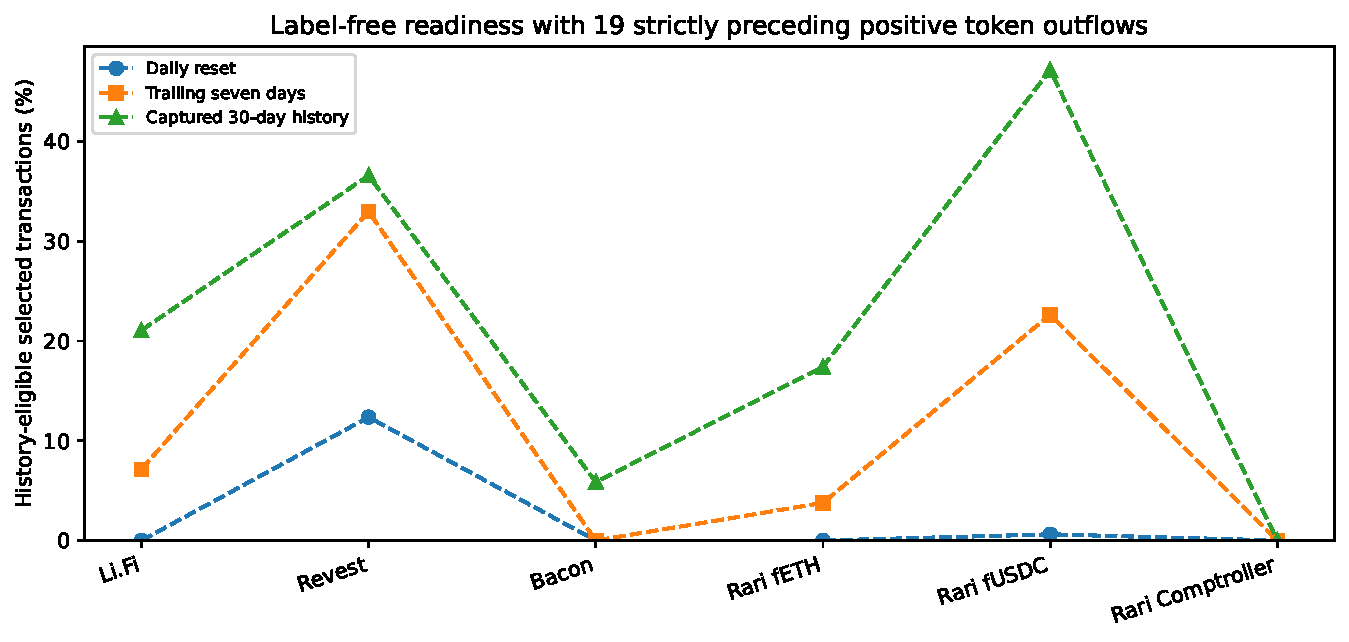
\includegraphics[width=\linewidth]{fig2_history_eligibility_six_views.pdf}
\caption{Label-free computability of token-outflow ranks in six fixed observation views under the same minimum-history rule. Different views are not independent samples from a defined population.}
\label{fig:readiness}
\end{figure}

A simple sensitivity analysis of minimum strictly preceding history lengths 1, 5, 10, 19 and 39 is reported as a machine-readable table for each view and initialization policy. This is \emph{not} a retrospective optimization of a detector threshold: the corresponding score triggering and exact-execution comparisons retain the original history minimum of 19. The sensitivity exposes how much workload remains eligible under alternative preconditions rather than suggesting an improved detection rate.

\subsection{Attack-time readiness, not end-of-day volume}
The additional Bacon/Rari audit allowed us to distinguish the number of selected transactions by the end of the incident day from those that precede the known exploit. Table~\ref{tab:attacktime} directly addresses a possible selection bias in the earlier source-only audit: reporting only days with less than 20 transactions conceals attack days with late traffic spikes. In fact, three of four component views record 20 or more selected transactions over the full incident day, but \emph{none} has 19 selected transactions strictly before the reference execution. The reference transaction itself is scored before its positive amount is appended to history.

\begin{table}[htbp]
\centering\footnotesize
\caption{Selected transactions on the documented attack day. The current execution is excluded from strictly preceding history. Four views belong to only two incident families.}
\label{tab:attacktime}
\begin{tabular}{lrrrrp{2.5cm}}
\toprule
View & Full day & Before & Ref. & After & Max earlier positive same-token values \\
\midrule
Bacon proxy & 23 & 2 & 1 & 20 & 0 \\
Rari fETH & 19 & 8 & 1 & 10 & 7 \\
Rari fUSDC & 48 & 17 & 1 & 30 & 11 \\
Rari Comptroller & 24 & 18 & 1 & 5 & 0 \\
\bottomrule
\end{tabular}
\end{table}

\begin{figure}[htbp]
\centering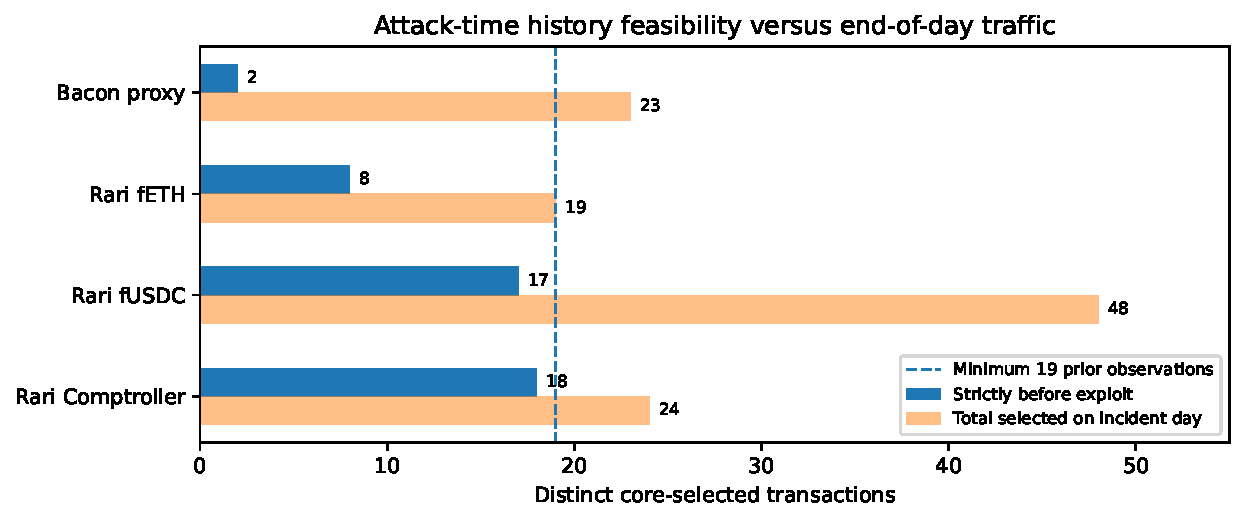
\includegraphics[width=\linewidth]{fig1_attack_time_selected.pdf}
\caption{Source-validated distinct transactions strictly before the documented execution (dark bar) versus the full day including the execution and subsequent traffic (light bar). The dashed line denotes the necessary 19 preceding selected transactions; the stricter feature-specific condition requires 19 earlier \emph{positive same-token outflows}.}
\label{fig:attacktime}
\end{figure}

This distinction is important for empirical software validation. A precondition that holds only after the event to be detected is not satisfied at the decision time. The last column gives the stronger token-specific result obtained from the selected complete-bundle reconstruction. It confirms that none of these four component views supplied 19 prior positive same-token outflows at the known execution. Therefore all four original daily-reset semantic misses have a measured feature-eligibility explanation, not merely an end-of-day event-rate argument. This observation does not establish what an alternative, independently chosen feature or a longer pre-window history would do.

\subsection{Source-level transportability across sixteen additional nominations}
The frozen incident-derived source screen successfully completed all sixteen 30-day windows (480 emitter-days), with exact original-Parquet source projections for 44,780 distinct case-specific selected transactions. Source acquisition recorded 4,827 accepted HTTP byte ranges and 4,262,470,409 response bytes; these are transport-accounting values and not a throughput benchmark. Every case had 30 accepted days, and no failed day was imputed as zero. The resulting case and daily tables, including original source keys and ETags, are permanently archived with the code and SHA-256 receipt ledger.

Across the 480 emitter-days, 302 had zero selected transactions, 108 had 1--19 and 70 had at least 20. Thus 410/480 days (85.42\%) fail the elementary necessary transaction-count condition. The number 410 is not evidence of a universal DeFi limitation, because some zero days may predate contract deployment. Conditioning \emph{only} on the 178 days containing at least one selected transaction yields 108/178 (60.67\%) with fewer than 20 transactions. The study does not certify these as days of active deployed contract operation or measure the stricter count of positive same-token outflows. A whole-window median obscures sharp within-case heterogeneity: Ronin's nominated Ethereum bridge and the Beanstalk proxy surpass 20 transactions on every source day, whereas the Schnoodle token does not do so on any of its 29 active source days. These results characterize selected source streams, not incident detection rates.

\begin{table}[htbp]
\centering\small
\caption{Independent source audit across sixteen fixed PoC-derived emitter windows. Each day is counted once per nomination. Zero activity cannot distinguish undeployed, inactive and silent contracts without further deployment evidence.}
\label{tab:newframe}
\begin{tabularx}{\linewidth}{@{}>{\raggedright\arraybackslash}X r r@{}}
\toprule
Emitter-selected transactions in UTC day & \shortstack{Contract-\\days} & \shortstack{Share of 480\\days}\\
\midrule
Exactly zero & 302 & 62.92\%\\
From 1 to 19 & 108 & 22.50\%\\
20 or more & 70 & 14.58\%\\
\midrule
All days & 480 & 100.00\%\\
\bottomrule
\end{tabularx}
\end{table}

\begin{figure}[htbp]
\centering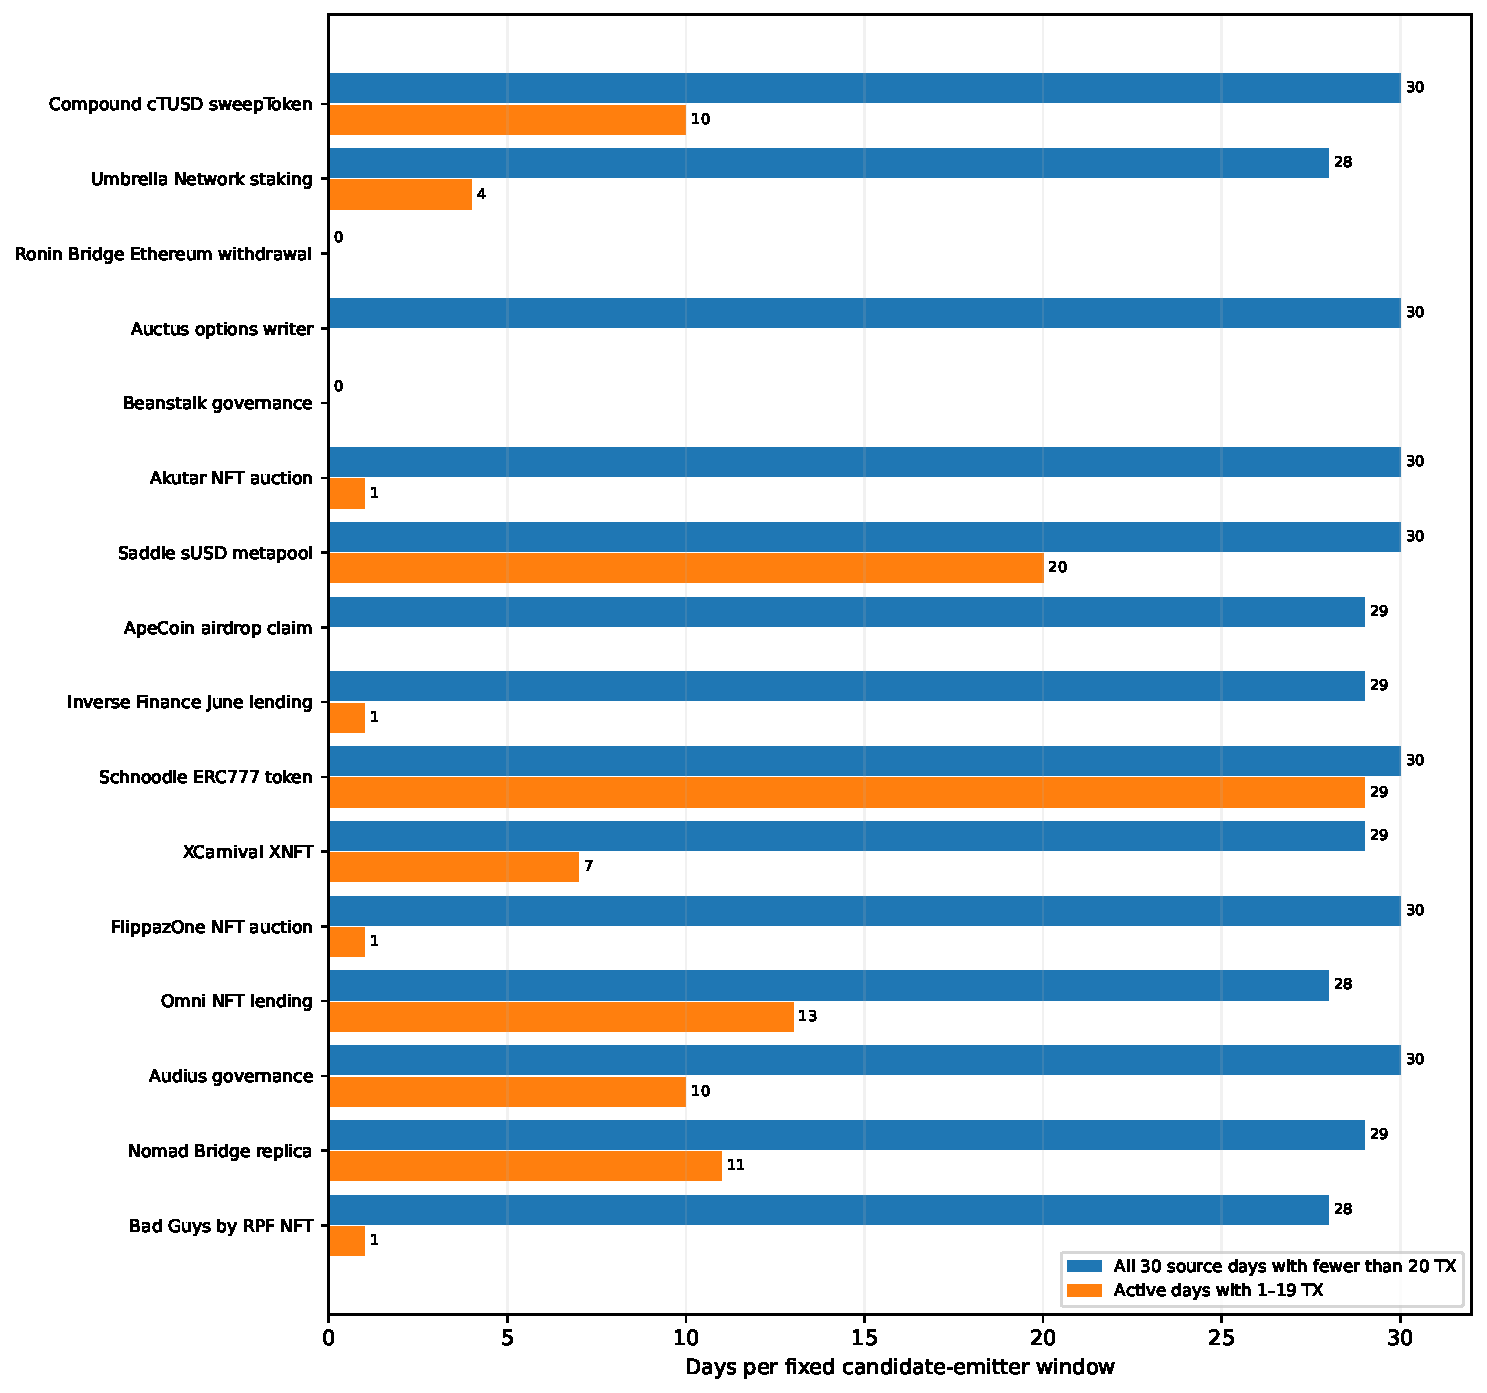
\includegraphics[width=\linewidth]{fig4_external_readiness_census.pdf}
\caption{For each frozen incident-derived nominated emitter, days with fewer than 20 selected transactions among all thirty source days (upper bar) and among the days with at least one selected transaction (lower bar). These are necessary feasibility bounds, not measured ERC-20 ranks or verified exploit detection.}
\label{fig:newframe}
\end{figure}

A separate, non-adjudicating transaction-reference preflight checked seventeen reported or PoC-associated Ethereum hashes spanning twelve of the sixteen nominations. All seventeen were indexed with successful execution status, but five are not fully matched to the nominated core source boundary: four have no indexed log from that emitter and one has an incomplete paginated log-bundle retrieval. Two candidate reference dates fall outside their \emph{PoC-fork-block-anchored} 30-day source window, including the Beanstalk exploit on 17 April versus a frozen source-window end of 16 April. This discrepancy validates the need to distinguish a reproducible PoC-fork source window from a legally admitted historical exploit window. None of these seventeen identity checks is counted as a newly accepted detector hit or miss; independent incident-role adjudication, appropriate time-window reassignment and complete selected log/status evidence are still required.

\subsection{RQ2: history initialization, count comparator and exact notifications}
Table~\ref{tab:outcomes} compares exact known-reference notifications with the total number of emitted messages under the primary greedy daily budget. An entry such as $1/3$ means that one known reference execution was notified in a three-alert stream; it is \emph{not} an estimate of precision. The count comparator is independent of rank-history mode and appears as its own reference column.

\begin{table}[htbp]
\centering\scriptsize
\caption{Primary outcomes as \emph{exact known-execution hits / all emitted notifications} (greedy, $B=5$, rank threshold $1/20$). No unknown notification is treated as a false positive. Three Rari views share one historical execution.}
\label{tab:outcomes}
\begin{tabular}{lrrrr}
\toprule
View & Semantic daily & Semantic 7 d & Semantic 30 d & Count daily \\
\midrule
Li.Fi core & 0/0 & 0/0 & 0/2 & \textbf{1/1} \\
Revest core & 0/0 & 0/2 & 0/1 & 0/2 \\
Bacon proxy & 0/0 & 0/0 & \textbf{1/1} & 0/1 \\
Rari fETH & 0/0 & \textbf{1/1} & \textbf{1/3} & 0/0 \\
Rari fUSDC & 0/0 & \textbf{1/2} & \textbf{1/7} & \textbf{1/2} \\
Rari Comptroller & 0/0 & 0/0 & 0/0 & \textbf{1/1} \\
\bottomrule
\end{tabular}
\end{table}

The original negative outcome persists for Li.Fi and Revest: greater historical readiness yields additional alerts but no exact known execution notification. Li.Fi's cumulative replay yields two unadjudicated notifications, on 1 and 3 March 2022, preceding the 20 March exploit. The Revest seven-day mode yields two unadjudicated notifications on 23 and 24 March, and cumulative history yields one on 24 March. These are not credited as early detections because no independently established relation to the attack has been shown.

By contrast, the new case results differ. Bacon's cumulative within-window history yields a reference-execution notification at 12:46:23 UTC on 5 March 2022: the USDC rank is $1/33$ after 32 strictly preceding positive core-outflow values. The trailing-seven-day history contains only five such values and cannot score that transaction. In Rari fETH, the known execution is notified under seven-day and cumulative histories with scores $1/24$ and $1/42$. In Rari fUSDC, independently recomputed seven-day scores are $1/27$ for USDC (26 previous observations) and $1/23$ for fUSDC (22 previous observations); the respective captured-window scores are $1/64$ (63 previous) and $1/34$ (33 previous). The two tokens are scored on one view of the same known Rari transaction, not independent incident hits. The Comptroller has no positive core-boundary token outflow, so no semantic trigger occurs, while the count comparator notifies the known execution. These are observation-view-dependent matches on one shared Rari execution, not multiple independent attacks.

Across all primary 1/20 cells in the new two-family replay, the offered budget never blocks an eligible grouped semantic candidate. Under the more permissive rank $1/10$, grouping and allocation can change realized loads; all retained policy/budget cells remain available in the result export. The main outcome is therefore driven principally by feature readiness, component observation and rank extremeness rather than budget exhaustion. Budget studies on the separate, previously exposed Euler and Beanstalk development workloads are not pooled into this external table; their event-time allocation findings answer a different question.

\subsection{Exploratory replay across seven further historical emitter views}\label{sec:sevenviews}
Table~\ref{tab:sevenstreams} presents the seven additional streams under the \emph{same} greedy daily budget ($B=5$). The three history modes change only the token-rank state; the core-event-count comparator has no history initialization. Every source-bound, selected transaction has a verified historical identity, and event payloads were obtained from a separate indexed source. The confirmed case selection was nonrandom and the reference sets do not exhaust each attack campaign, so the final column is an \emph{exact join to documented candidate transactions}, not complete incident recall.

\begin{table}[htbp]
\centering\scriptsize
\caption{Seven additional nominated emitter windows. Rank columns are daily reset / trailing 7 d / cumulative in captured 30 d. \emph{Ready} is the number of selected transactions with any eligible rank-1/20 score; \emph{alerts} are emitted notifications (greedy, $B=5$). Exact joins are conditional on an incomplete documentary candidate inventory; a dash means no reference was independently accepted for joining.}
\label{tab:sevenstreams}
\setlength{\tabcolsep}{4pt}
\begin{tabularx}{\linewidth}{@{}>{\raggedright\arraybackslash}X r c c r l@{}}
\toprule
Fixed emitter view & Selected TX & Ready (d/7/30) & Rank alerts (d/7/30) & Count alerts & Documented exact join \\
\midrule
Umbrella & 92 & 0/0/0 & 0/0/0 & 0 & --- \\
Saddle & 44 & 0/0/3 & 0/0/0 & 1 & 0/1 \\
Inverse & 71 & 20/20/20 & 3/3/3 & 2 & 0/1 \\
Schnoodle & 134 & 0/0/0 & 0/0/0 & 27 & \textbf{1/1 (count)} \\
XCarnival & 43 & 0/0/0 & 0/0/0 & 4 & 0/1 selected \\
Omni & 103 & 0/0/0 & 0/0/0 & 5 & 0/1 \\
Audius & 38 & 0/0/0 & 0/0/0 & 0 & 0/3 selected \\
\midrule
Total & 525 & --- & --- & --- & Nonindependent \\
\bottomrule
\end{tabularx}
\end{table}

No nominal rank history is computable for the selected Umbrella, Schnoodle, XCarnival, Omni or Audius streams under any tested initialization. In the nominated Saddle metapool, three selected transactions acquire an eligible token rank only with retained history, but none crosses the fixed trigger threshold. The Inverse yvCrv view has twenty history-eligible transactions in every state mode and three emitted rank notifications, yet none coincides with the separately documented June 16 exploit execution \citep{BlockSec2022Inverse}. Thus more history is neither necessary nor sufficient to generate a confirmed reference match: the observed token amount still must be an upper-tail extreme at the nominated contract boundary and must survive grouping and dispatch.

The count comparator produces a qualitatively different result on Schnoodle. It emits 27 notifications in that 30-day selected-token-proxy stream; one coincides exactly with the reported June 18 execution \citep{Schnoodle2022Analysis}. The other 26 have not been independently assigned benign or malicious truth, and 1/27 is \emph{not} measured precision. Similarly, XCarnival involves two documented candidate stages, but only one appears in the fixed XNFT-proxy selection: a later lending/borrow stage emits no XNFT event under this boundary. The Audius candidate inventory spans four governance/setup/asset-sale stages, one of which has no nominated governance-emitter event; none is notified by either simple rule \citep{XCarnival2022Account,Audius2022Report}. These cases substantiate why the monitor's source-level selection and attack construct must be evaluated separately.

Across this seven-case extension, all 441 method-policy configurations were cross-checked using two independently authored scoring implementations and had identical emitted transaction sequences. Multiple alerts, alternative initializations and budget settings in the same view are correlated, not additional incidents. No claim of label completeness or prospective deployment benefit follows from their agreement. The \emph{primary} four-family analysis and this \emph{exploratory extension} remain separate in the reported denominators.

\subsection{Alert timing and reference status}
An auditable notification result requires the exact notified transaction identity and its associated score, not only a total count. We generated a 19-row primary semantic notification ledger from the original score streams, independently reconstructed historical decisions and the fixed reference inventories. Every record contains source case/view, UTC event time, token identity, rank, initialization, the emitted transaction hash and one of two reference statuses: independently verified known execution or \emph{unadjudicated}. The complete ledger is retained in the companion artifact and a compact reading of the results appears in Appendix~\ref{app:alerts}.

\begin{figure}[htbp]
\centering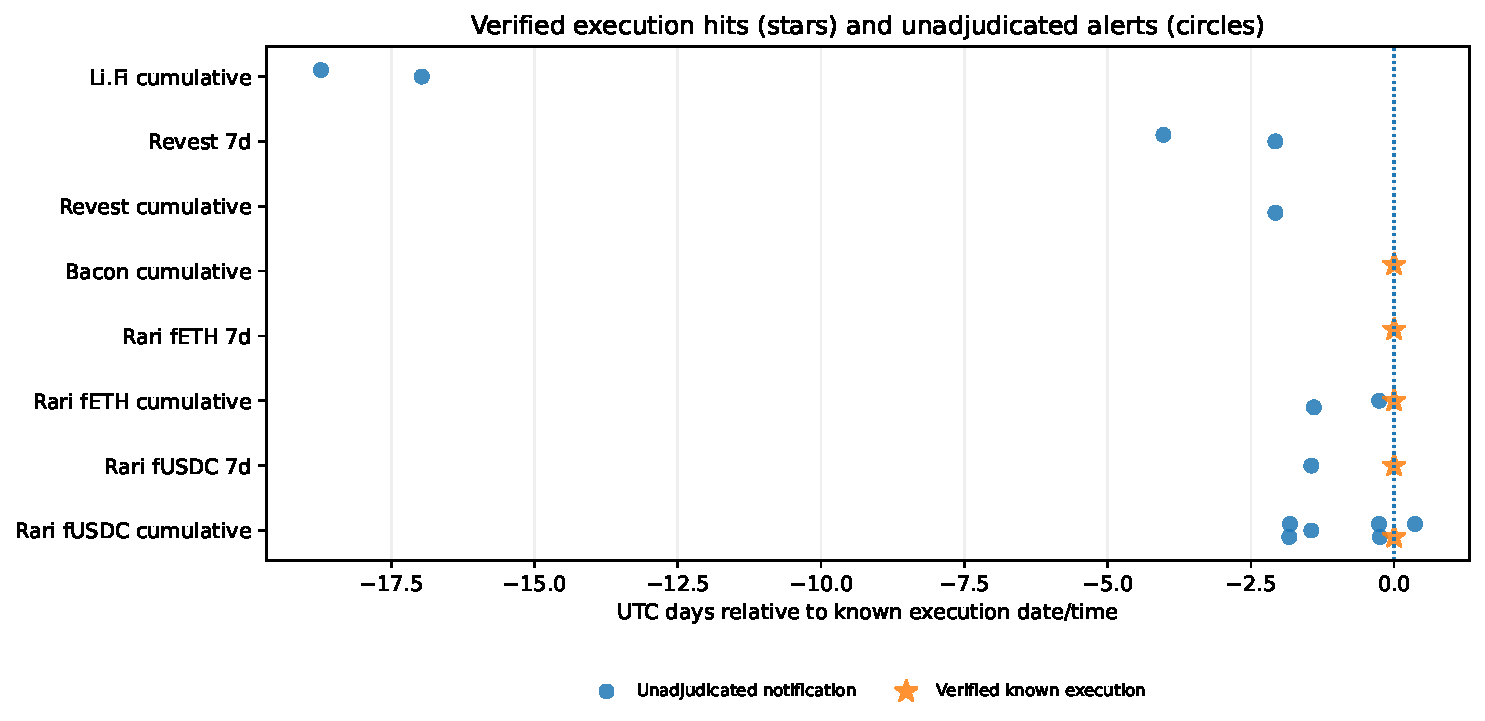
\includegraphics[width=\linewidth]{fig3_incident_relative_alerts.pdf}
\caption{Timing of primary semantic notifications relative to the documented execution time. Stars mark notifications on the exact admitted reference, and circles denote unadjudicated notifications. Rari rows share the same reference execution; Li.Fi and Revest reference times come from the independently admitted historical identities. A small deterministic vertical displacement separates overlapping plotted notifications without changing their time coordinates. The graph does not establish early warning or live notification latency.}
\label{fig:alerttime}
\end{figure}

The nonreference notifications should be investigated separately if precision or actionable triage cost is to be evaluated. Labelling the unadjudicated alerts as false positives merely because they are not the single known execution would bias the result. Equally, the presence of an alert before an exploit date does not demonstrate the alert's causal relevance to the later event.

\subsection{RQ3: feature--mechanism correspondence}
The original Li.Fi post-mortem and independent attack analysis describe an external-call/approval route: user funds could be transferred through allowances granted to the protocol \citep{LiFi2022Postmortem,BlockSec2022LiFi}. The reference transaction contains 40 ERC-20-shaped logs, of which only three touch the monitored diamond core; 92 logs were emitted across the transaction. The positive USDC/USDT core-boundary flows used by the rank rule are not the victim-to-attacker transfers themselves. With cumulative history, the Li.Fi USDC rank on the reference is $54/56$, not a high-outflow anomaly. This is a construct limitation independent of the original daily-history ineligibility.

Revest's admitted reference tokens have no strictly preceding positive outflows in the retained 30-day history, despite positive flows at the known executions; its documented exploit relates to reentrancy and FNFT accounting rather than an isolated magnitude tail \citep{Revest2022Postmortem,SlowMist2022Revest}. In Bacon, an exact rank notification appears under cumulative history, but a positive USDC transfer at the lending proxy is not by itself proof that the statistic recognizes the underlying reentrancy mechanism. In Rari, the fETH token outflow event and fUSDC ERC-20 transfer patterns are similarly not interchangeable with the principal native-ETH borrowing/state update exploit mechanism documented by the team \citep{Rari2022Postmortem}. Exact transaction coincidence is measurable and meaningful; precise exploit-mechanism recognition is a stronger claim that these syntactic features do not establish.

The source-tier, component-role and token/transaction distinctions thus matter to requirements engineering for a monitor. Before treating a rule as an exploit detector, a specification must state which class of adversarial state transition the feature is intended to represent, which contracts must be observed, and whether the feature is available strictly before the requested decision. This does not turn the studied rank statistic into a new attack-specific detector.

\section{Discussion: implications for reliable monitoring software}\label{sec:discussion}

\subsection{A testable chain of necessary conditions, not a sufficient attack oracle}
The case evidence motivates a falsifiable four-stage contract. \emph{A: observation alignment}: the nominated contract boundary must carry a positive gross ERC-20 outflow relevant to the hypothesized mechanism. \emph{B: readiness}: the same token must have at least 19 strictly prior positive outflows in the specified retained history. \emph{C: conditional extremeness}: the current gross amount must satisfy $r\leq1/20$. \emph{D: dispatch}: the raw trigger must pass candidate grouping and daily notification admission. These properties can be checked independently from the incident label, then joined to a known execution. \textbf{A and B are necessary but not sufficient for a rank alert}; passing them does not establish exploitation, a high conditional rank, or a delivered notification. A measurement program that conflates readiness with accuracy cannot attribute the observed failure correctly.

\begin{table}[htbp]
\centering\footnotesize
\caption{Necessary feature conditions at known executions. Rari views share the same transaction. A/B do not ensure that rank C passes or that an alert is emitted.}
\label{tab:abc}
\setlength{\tabcolsep}{3pt}
\begin{tabularx}{\linewidth}{p{2.0cm} >{\raggedright\arraybackslash}X p{1.72cm} >{\raggedright\arraybackslash}X}
\toprule
View & A: observed boundary & B: previous samples & C: rank; exact hit \\
\midrule
Li.Fi & Core flow misses user approval drain & USDC: 55 & $54/56$; no \\
Revest & Token outflows present & RENA/ECO: 0 & Undefined; no \\
Bacon proxy & USDC core outflow & USDC: 32 & $1/33$; cumulative \\
Rari fETH & Positive core outflow & fETH: 23 (7d) & $1/24$; 7d, cumulative \\
Rari fUSDC & Positive ERC-20 outflow & USDC 26/63; fUSDC 22/33 & 7d: $1/27$, $1/23$; 30d: $1/64$, $1/34$; hit \\
Rari Comptroller & No positive ERC-20 core outflow & None & Undefined; count hit \\
\bottomrule
\end{tabularx}
\end{table}

The coincidence of an exact alert and an incident transaction is a label-linked outcome, not proof that the outflow magnitude captures reentrancy or any other causal exploit semantics. Likewise, no positive gross outflow at one observation boundary does not imply absence of any native-value transfer elsewhere in the transaction. This contract separates a \emph{monitor validation check} from a security-classification claim and predicts where a monitored feature will be undefined, where it will be defined but unexceptional, and where the notification stage will become the next possible point of failure.

\subsection{From an eligibility check to a validation obligation}
The inequality $N_{k,d}\geq20$ is not intrinsically a research contribution: it follows directly from the rank rule's configured minimum history. Its engineering value depends on measuring the \emph{right} $N_{k,d}$ from available data, applying it at the decision time and using it to avoid invalid comparisons. The accepted experimental records demonstrate a sequence of increasingly restrictive checks: daily emitted log counts, unique selected transaction counts, positive same-token outflows, and strictly preceding history at the reference execution. Each stage excludes conclusions that would have appeared plausible from the weaker count alone.

This hierarchy is an executable monitor requirement. A deployment or evaluation report should distinguish ``no candidate because score below threshold'' from ``no candidate because score was ineligible'' and from ``unknown because source observation failed.'' Our results show why reporting only the total number of alerts obscures these categories. A program that emits zero alerts may be correctly implementing its alert cap while being unable to run the anomaly statistic. Model and software assurance should make those states explicit rather than encode them as normal observations.

The phenomenon is not confined to one date or code path in this cohort: Li.Fi and Revest have different token-history distributions; the Bacon and Rari records likewise show markedly different conditional score availability across nominated component views. The full attack-day transaction count can also be misleading, because many selected transactions occur after the exploit. This reinforces the requirement to measure historical state causally before each evaluated event. The present sample does not justify extrapolating these fractions to every DeFi contract or to all history-dependent detectors.

\subsection{A history intervention can restore a hit, but not consistently}
Initialization cannot be evaluated by counting newly eligible transactions alone. Under the same rank rule, Li.Fi and Revest gain history-eligible transactions without new known-execution notifications; Bacon and two Rari component views obtain known-execution matches. Longer history changes not only the number of previous observations but also the empirical rank of a given current amount. Consequently raw-trigger count need not increase monotonically with available history, even though eligibility generally increases. At Rari fETH, for example, the current known execution is an extreme value relative to both seven-day and cumulative histories, whereas the Li.Fi observed core-boundary USDC amount is not.

These comparisons are \emph{counterfactual historical replays}, not randomized experiments and not measured prospective deployment outcomes. Both the revised modes and the new case study arose after the initial two-case results were known; historical core nominations were incident-informed. A new independent cohort with a frozen eligibility preflight and blinded scoring is necessary before interpreting differences as generalizable. In particular, a single Rari transaction scored against three component views cannot be counted three times in a significance test.

\subsection{Transferability of feature-domain failures}\label{sec:transport}
The broader source evidence distinguishes three quantities that could otherwise be conflated: \emph{traffic feasibility} (enough selected transactions to populate a history), \emph{feature computability} (sufficient qualifying observations and a valid score domain), and \emph{security correspondence} (the recorded quantity describes the exploit-relevant operation). The sixteen-entry S3 census measures only the first quantity. The twelve comparison-contract windows show that even active monitors can have sharply different score domains: with identical discrete core-log-count observations and daily resets, a 19-observation z-score is defined in 38.50\% of transactions, a positive-MAD statistic in 1.93\%, and a 5-observation EWMA in 99.52\%. The seven additional transaction-level streams then recover the token-outflow domain on specific emitter views. Five show zero rank-ready transactions across all tested state modes; Saddle retains three eligible observations without any rank alert; Inverse has eligible scores and alerts but no documentary reference join. This layered evidence is stronger than the tautological inequality $N\geq20$, because the measured failure changes with feature choice, emitter role and event-time alignment.

Schnoodle, Li.Fi, and the Rari Comptroller view further illustrate complementarity between a core-event-count alert and a token-amount rank: they may match a documented execution through count despite the rank's missing domain, while Bacon's known match appears only through the historical amount rank. This is an engineering argument for explicitly validating the feature's domain and retaining diverse signal types, \emph{not} a demonstration of ensemble superiority. The count rule's 27 alerts on Schnoodle also establishes an unresolved operator-load trade-off rather than a defensible false-positive count. Because the original history policy and event boundary were not prospectively randomized across protocols, no causal, population-wide efficiency or attack-prevention claim is warranted.

\subsection{Implications for reliable monitor engineering}
A dependable monitoring system should state and test its observation boundary, prior-state availability, feature domain, grouping and dispatch requirements as explicit contracts. A successful unit test of the rank formula is not an acceptance test for an operational monitor. Component-level validation should report \emph{undefined} scores separately from low anomaly scores and should test state initialization under causal event time. The mixed outcomes here also caution against treating a count-only rule and an amount-rank rule as substitutes: exact Li.Fi and Rari Comptroller notifications arise from the count comparator, whereas the Bacon exact match arises from the accumulated token-outflow rank. This is complementarity of feature sensitivities in these selected traces, not evidence of general benefit from an ensemble.

The comparison-contract census shows why count sufficiency alone is a poor substitute for feature readiness. Among more than 714,000 observations, a five-sample EWMA is almost always defined, whereas a positive-MAD statistic on the same discrete core-log count is undefined in approximately 98\% of daily-reset observations. In the separate sixteen-emitter frame, 108 of 178 nonempty emitter-days contain fewer than 20 selected transactions. These samples differ by protocol role and construction, so their rates are descriptive rather than a matched estimate of population prevalence. Whether actual ERC-20 outflow histories are computable remains an independent measurement obligation. Future software-monitor benchmarks should stratify contracts by role, transaction activity and feature observability before scoring attacks, rather than sample only from detectable or attack-rich cases.

\subsection{Practical evaluation checklist}
Before claiming that a monitor detects a given class of incidents, an evaluator should: define the relevant state transition and observable contracts; establish that source partitions and selected all-emitter bundles are available; compute the fraction of observations for which every required feature is defined; measure state readiness \emph{at} the reference execution; report candidate grouping and realized alerts separately; and join a documented reference inventory only after decisions are fixed. Applying these checks does not guarantee detector quality, but their omission can produce uninterpretable detection statistics.

\subsection{Source-verified alert audit and scope of unresolved labels}
The primary rank-$1/20$ ledger contains 19 emitted view-specific notifications. Fourteen do not match the limited admitted reference inventory; they represent twelve distinct transactions and eight distinct direct sending addresses. Two Rari senders each appear in three unadjudicated transactions: one called \texttt{mint} and \texttt{redeemUnderlying}, the other repeatedly called \texttt{redeemUnderlying}. None of these eight direct senders equals the independently reported Rari attack sender; indirect control or preparation cannot be ruled out. Two unadjudicated Li.Fi notifications share the diamond recipient address with the known execution, which merely establishes a call to the same monitored contract. The indexed metadata do not establish maliciousness, benignity, complete attacker identity or pre-attack warning. Notification counts reflect emitted workload, not a measured false-positive rate or analyst time.

For all ten distinct Bacon/Rari transactions in the primary rank-$1/20$ notification ledger, an independent source-level comparator obtained their complete \texttt{topics}, \texttt{data}, emission order and log address from the original AWS historical Parquet objects and found exact equality with the normalized Blockscout log contents. The resulting source-hash ledger, HTTP range receipts and versioned verification code are retained in the original-source verification artifact. This reduces the risk of indexer-only event-payload disagreement for the decisive transactions. It does not independently certify statuses, all 667 selected transactions, full incident reference inventories or receipt roots. The public repository's normalized historical input and replay archives were subsequently checked by a clean-workspace independent reproduction workflow, making an expiring GitHub Actions download unnecessary for reproducing the reported decisions.

\section{Threats to validity}\label{sec:validity}

\paragraph{Case selection and statistical independence.} Four incident families were studied in the primary analysis, with five successful executions admitted to known subsets. A separate nonrandom, source-constrained extension scored seven further fixed emitter windows (525 selected transactions; 441 dependent policy cells), but did not close complete historical incident references. Li.Fi and Revest were previously exposed, Bacon and Rari were selected after these results, and component nominations were incident-informed. One Rari execution is represented in multiple component views. The study neither estimates a population recall nor applies significance tests across deterministic replay configurations. The sample cannot establish universality or comparative superiority. The selection of one Bacon proxy and one Rari pool is a source-availability decision, not a representative sampling mechanism. The twelve extra comparison-contract emitters were similarly nonrandom, not matched on role or deployment date, and not verified benign. Differences between them and incident-selected cores can reflect contract role, traffic composition or sampling, rather than any intrinsic attack association.

\paragraph{Reference completeness and unadjudicated alerts.} The incident reports do not close every attack-execution inventory, especially for Rari's multiple affected pools. Additional exact reference candidates in the earlier cases retain unresolved roles. Alerts not matching the admitted known execution are not labelled benign. Hence precision, false-positive rate, missed economic loss and complete incident-level failure cannot be inferred.

\paragraph{Provenance and observation boundary.} The first two families have original S3-based selected transactions and separately audited replay input. For Bacon, Rari and the seven additional source-bound streams, selected transaction identities and core-emitter counts were checked against original Parquet objects, while most complete event topics/data and success statuses were supplied by a distinct historical indexer. The latter data were independently checked against complete original AWS event payloads for all ten distinct Bacon/Rari transactions in the primary notification-and-reference ledger, but not for all 667 selected transactions or against Ethereum receipt roots. Contract address nomination and event-typed arithmetic may also omit native ETH, internal calls, token-specific semantics or state invariants. Data missing from a view cannot be taken as evidence that an exploit did not occur.

\paragraph{Temporal state and operational interpretation.} Three score-history modes start from a truncated, retained 30-day observation window. The seven-day mode is a trailing lookback within that source boundary; the cumulative mode lacks pre-window history. All grouping and budget states reset at UTC midnight by design. The historical timestamps are block event times, not observed availability or notification latency. Even an exact notification on an atomic exploit transaction does not establish any ability to prevent that transaction or reduce its loss.

\paragraph{Implementation and measurement verification.} Independent re-evaluation reproduced all newly accepted score/candidate/notification configurations and the earlier sealed comparisons. These checks constrain implementation disagreement but cannot prove the truth of all incident narratives or the completeness of a third-party indexer. Our readiness-sensitivity analyses do not represent optimized alternative detector parameters. Reproducing the decisions also does not provide a controlled performance benchmark or a study of operator response burden.

\section{Conclusion}\label{sec:conclusion}

We examined a fixed history-dependent token-outflow monitor as a software system with observation and state contracts, rather than assuming that a defined threshold implies an executable detector. Across four retrospective Ethereum incident families, the original daily-reset rank rule produced no exact known-execution notification on the admitted reference set. In the newly reconstructed Bacon and Rari cases, only 2, 8, 17 and 18 view-selected transactions, respectively, preceded the documented exploit on its UTC day; end-of-day totals masked this deficit. Full replay of strictly prior seven-day and captured-window histories produced contrasting outcomes: Li.Fi and Revest gained unadjudicated notifications without new known-execution matches, whereas Bacon and Rari acquired exact matches under longer-history variants. A count baseline also matched documented executions in some views. The implications are specific to the chosen feature, contracts and incident subsets, not a superiority claim.

The defensible general lesson for monitoring-software evaluation is to report feature computability, history state, construct alignment, conditional rank extremeness, and actual emitted notifications as separate measurable quantities. The separate comparison-contract sample quantifies that readiness depends on the feature definition: daily-reset rolling z-score, positive-MAD and EWMA warm-up were computable on 38.50\%, 1.93\% and 99.52\% of 714,951 emitter-log-count observations, respectively. The independent PoC-derived emitter source census adds 16 fixed component windows and 480 source days; only 70 days reached twenty selected transactions, and 108 of 178 nonempty emitter-days did not. A source-bound, nonrandom seven-stream follow-up reconstructed 525 selected transactions and independently reproduced 441 fixed-policy configurations. It found a count-based exact join on one documented Schnoodle execution amid 27 notifications, while the amount-rank rule remained ineligible in that fixed token view. The remaining nominated streams exhibited distinct readiness and boundary constraints. These results are exploratory, do not establish population prevalence, incident-wide recall or FPR, and do not turn the sixteen source-census entries into sixteen accepted detection trials. We provide source-linked identities, independent calculation checks and a traceable alert ledger for these claims. A broader prospective cohort, complete reference inventory and comparison against additional monitor definitions are necessary to establish cross-protocol generality.

\section*{Data, code and reproducibility}
The original sealed baseline remains \href{https://github.com/KuznetsovKarazin/blockchain-analytics-lab/commit/e720697bc3986dd291a7047c580cf973ae6e5567}{\texttt{e720697}}. The Li.Fi/Revest and Bacon/Rari normalized original input archives, independent source verifiers and comparison-contract data are publicly retained under \texttt{papers/monitoring\_jss/phase16--27}. The sixteen-entry Phase28 candidate source registry, all 480-day derived counts, and the 7-stream source-matched and independently verified observations/notifications are in \texttt{papers/monitoring\_jss/phase28--30}. These directories include original AWS transaction-identity SHA-256 receipts, Blockscout-indexed full event bundles, and exact independent method-policy comparison across 441 configurations. The source-pinned repository is \url{https://github.com/KuznetsovKarazin/blockchain-analytics-lab/tree/research/monitoring-v6-independent-cohort}; the immutable evidence snapshot and paper source are identified by the final release reference \texttt{article2-jss-v6.1-2026-10-29} once published. The precise commit and its file manifest are given in the accompanying reproducibility README. No Zenodo DOI has been assigned. Further provenance restrictions follow from the difference between original AWS event identities and Blockscout-supplied topics/data/status. Permissions and final author declarations must be confirmed before submission \citep{Kuznetsov2026Artifacts}.
\section*{Competing interests}
\textit{Author confirmation required before submission.}
\section*{Funding}
\textit{Author confirmation required: identify only grants that actually supported the reported work, with the required agreement numbers.}
\section*{Declaration of generative AI and AI-assisted technologies in the manuscript preparation process}
During preparation of this work, OpenAI ChatGPT (GPT-6) and OpenAI Codex were used to assist with literature organization, code drafting, checking reproducibility, scientific language editing, and LaTeX composition. The outputs were subjected to source comparison and deterministic tests as described in Methods. The author must review and edit the final manuscript and code as needed and take full responsibility for the content of the submitted article. \textit{Author confirmation of the exact tools used and this statement is required before submission.}

\appendix
\section{Complete primary notification ledger}\label{app:alerts}
Each row corresponds to one emitted semantic notification in the primary rank-$1/20$, greedy, $B=5$ comparison. Token names are indicative addresses mapped to common token symbols only where their identity is unambiguous; the downloadable CSV retains full contract addresses, scores and transaction hashes. \textbf{Known} means an exact match with an admitted successful execution. \textbf{Unknown} means the notification has not been independently adjudicated and must not be classified as a false positive.

\begingroup\scriptsize\setlength{\tabcolsep}{3pt}
\begin{longtable}{p{1.85cm}p{1.0cm}p{2.3cm}p{3.0cm}p{1.2cm}}
\caption{Exact emitted-transaction ledger for the primary rank rule (greedy, $B=5$). Multiple entries at the same transaction represent alternative component-view simulations, not separate attacks.}\label{tab:alerts}\\
\toprule
View & History & UTC date and time & Triggering token(s) and rank(s) & Status \\
\midrule
\endfirsthead
\toprule
View & History & UTC date and time & Triggering token(s) and rank(s) & Status \\
\midrule
\endhead
Bacon & 30d & 2022-03-05 12:46 & USDC 1/33 & Known \\
Li.Fi & 30d & 2022-03-01 09:25 & USDC 1/20 & Unknown \\
Li.Fi & 30d & 2022-03-03 03:42 & USDC 1/22 & Unknown \\
Rari fUSDC & 30d & 2022-04-28 13:38 & USDC 1/53 & Unknown \\
Rari fUSDC & 30d & 2022-04-28 13:57 & USDC 1/27 & Unknown \\
Rari fUSDC & 30d & 2022-04-28 22:50 & USDC 1/58 & Unknown \\
Rari fETH & 30d & 2022-04-28 23:55 & fETH 1/30 & Unknown \\
Rari fUSDC & 30d & 2022-04-30 03:08 & fUSDC 1/24 & Unknown \\
Rari fETH & 30d & 2022-04-30 03:15 & fETH 1/37 & Unknown \\
Rari fUSDC & 30d & 2022-04-30 03:32 & fUSDC 1/25 & Unknown \\
Rari fETH & 30d & 2022-04-30 09:32 & fETH 1/42 & Known \\
Rari fUSDC & 30d & 2022-04-30 09:32 & USDC 1/64; fUSDC 1/34 & Known \\
Rari fUSDC & 30d & 2022-04-30 18:14 & USDC 1/37 & Unknown \\
Rari fUSDC & 7d & 2022-04-28 22:50 & USDC 1/22 & Unknown \\
Rari fETH & 7d & 2022-04-30 09:32 & fETH 1/24 & Known \\
Rari fUSDC & 7d & 2022-04-30 09:32 & USDC 1/27; fUSDC 1/23 & Known \\
Revest & 30d & 2022-03-24 23:57 & token 0x120a 2/64 & Unknown \\
Revest & 7d & 2022-03-23 01:04 & token 0x120a 1/20 & Unknown \\
Revest & 7d & 2022-03-24 23:57 & token 0x120a 1/57 & Unknown \\
\bottomrule
\end{longtable}
\endgroup


\section{Additional incident-derived source and reference checks}\label{app:sourcecensus}
\small
\begin{longtable}{@{}p{6.9cm}rrrr@{}}
\caption{Original-source selected-transaction census for the sixteen additional nominations. These are source-window counts anchored to PoC fork dates, not completed historical incident-detection evaluations.}\label{tab:allcensus}\\
\toprule
Candidate emitter & TX & 0 TX/d & 1--19/d & $\geq20$/d\\
\midrule
\endfirsthead
\toprule
Candidate emitter & TX & 0 TX/d & 1--19/d & $\geq20$/d\\
\midrule
\endhead
Compound cTUSD sweepToken & 15 & 20 & 10 & 0\\
Umbrella Network staking & 92 & 24 & 4 & 2\\
Ronin Bridge Ethereum withdrawal & 18,522 & 0 & 0 & 30\\
Auctus options writer & 0 & 30 & 0 & 0\\
Beanstalk governance & 12,392 & 0 & 0 & 30\\
Akutar NFT auction & 1 & 29 & 1 & 0\\
Saddle sUSD metapool & 44 & 10 & 20 & 0\\
ApeCoin airdrop claim & 10,938 & 29 & 0 & 1\\
Inverse Finance June lending & 71 & 28 & 1 & 1\\
Schnoodle ERC777 token & 134 & 1 & 29 & 0\\
XCarnival XNFT & 43 & 22 & 7 & 1\\
FlippazOne NFT auction & 1 & 29 & 1 & 0\\
Omni NFT lending & 103 & 15 & 13 & 2\\
Audius governance & 38 & 20 & 10 & 0\\
Nomad Bridge replica & 930 & 18 & 11 & 1\\
Bad Guys by RPF NFT & 1,456 & 27 & 1 & 2\\
\midrule
All sixteen & 44,780 & 302 & 108 & 70\\
\bottomrule
\end{longtable}
\normalsize

\begin{table}[htbp]
\centering\small
\caption{Indexer reference preflight for twelve of the sixteen incident-derived candidate families. All indexed hashes have successful status, but neither their exact role nor incident-wide completeness has been independently adjudicated. ``Core present is indexed log-emitter matching, not a detector notification; ``? indicates incomplete source pagination.}
\label{tab:refpreflight}
\begin{tabularx}{\linewidth}{@{}>{\raggedright\arraybackslash}X r r r@{}}
\toprule
Case & Indexed TX & Core present & Within PoC window\\
\midrule
Umbrella Network staking & 1 & 1/1 & 1/1\\
Beanstalk governance & 1 & 1/1 & 0/1\\
Akutar NFT auction & 1 & 0/1 & 0/1\\
Saddle sUSD metapool & 1 & 1/1 & 1/1\\
ApeCoin airdrop claim & 1 & 1/1 & 1/1\\
Inverse Finance June lending & 1 & 1/1 & 1/1\\
Schnoodle ERC777 token & 1 & 1/1 & 1/1\\
XCarnival XNFT & 2 & 1/2 & 2/2\\
Omni NFT lending & 1 & 0/1 (1 unknown) & 1/1\\
Audius governance & 4 & 3/4 & 4/4\\
Nomad Bridge replica & 2 & 1/2 & 2/2\\
Bad Guys by RPF NFT & 1 & 1/1 & 1/1\\
\midrule
All candidate references & 17 & 12/17 (1 unknown) & 15/17\\
\bottomrule
\end{tabularx}
\end{table}


\section{Additional measurement details}\label{app:measurement}
The independent source audit checked 60 daily log objects for Bacon and Rari component address membership and confirmed selected transaction identities across all 60 days. The later source tier used the Blockscout indexer for the complete contents and successful status of those selected transactions. The verification scripts reject missing cases, mismatched source identities, changed hashes and inconsistent counts. For each per-token rank, a transaction is scored against strictly prior successful observations and is inserted into the token history only after its own score is evaluated. No unlabelled notification is replaced by a labelled negative. Counts and timestamps in the main text were regenerated from the machine-readable result files, not manually transcribed from plots.

\bibliographystyle{elsarticle-harv}
\begingroup\footnotesize\sloppy\bibliography{references}\endgroup
\end{document}
